\documentclass[1p]{elsarticle_modified}
%\bibliographystyle{elsarticle-num}

%\usepackage[colorlinks]{hyperref}
%\usepackage{abbrmath_seonhwa} %\Abb, \Ascr, \Acal ,\Abf, \Afrak
\usepackage{amsfonts}
\usepackage{amssymb}
\usepackage{amsmath}
\usepackage{amsthm}
\usepackage{scalefnt}
\usepackage{amsbsy}
\usepackage{kotex}
\usepackage{caption}
\usepackage{subfig}
\usepackage{color}
\usepackage{graphicx}
\usepackage{xcolor} %% white, black, red, green, blue, cyan, magenta, yellow
\usepackage{float}
\usepackage{setspace}
\usepackage{hyperref}

\usepackage{tikz}
\usetikzlibrary{arrows}

\usepackage{multirow}
\usepackage{array} % fixed length table
\usepackage{hhline}

%%%%%%%%%%%%%%%%%%%%%
\makeatletter
\renewcommand*\env@matrix[1][\arraystretch]{%
	\edef\arraystretch{#1}%
	\hskip -\arraycolsep
	\let\@ifnextchar\new@ifnextchar
	\array{*\c@MaxMatrixCols c}}
\makeatother %https://tex.stackexchange.com/questions/14071/how-can-i-increase-the-line-spacing-in-a-matrix
%%%%%%%%%%%%%%%

\usepackage[normalem]{ulem}

\newcommand{\msout}[1]{\ifmmode\text{\sout{\ensuremath{#1}}}\else\sout{#1}\fi}
%SOURCE: \msout is \stkout macro in https://tex.stackexchange.com/questions/20609/strikeout-in-math-mode

\newcommand{\cancel}[1]{
	\ifmmode
	{\color{red}\msout{#1}}
	\else
	{\color{red}\sout{#1}}
	\fi
}

\newcommand{\add}[1]{
	{\color{blue}\uwave{#1}}
}

\newcommand{\replace}[2]{
	\ifmmode
	{\color{red}\msout{#1}}{\color{blue}\uwave{#2}}
	\else
	{\color{red}\sout{#1}}{\color{blue}\uwave{#2}}
	\fi
}

\newcommand{\Sol}{\mathcal{S}} %segment
\newcommand{\D}{D} %diagram
\newcommand{\A}{\mathcal{A}} %arc


%%%%%%%%%%%%%%%%%%%%%%%%%%%%%5 test

\def\sl{\operatorname{\textup{SL}}(2,\Cbb)}
\def\psl{\operatorname{\textup{PSL}}(2,\Cbb)}
\def\quan{\mkern 1mu \triangleright \mkern 1mu}

\theoremstyle{definition}
\newtheorem{thm}{Theorem}[section]
\newtheorem{prop}[thm]{Proposition}
\newtheorem{lem}[thm]{Lemma}
\newtheorem{ques}[thm]{Question}
\newtheorem{cor}[thm]{Corollary}
\newtheorem{defn}[thm]{Definition}
\newtheorem{exam}[thm]{Example}
\newtheorem{rmk}[thm]{Remark}
\newtheorem{alg}[thm]{Algorithm}

\newcommand{\I}{\sqrt{-1}}
\begin{document}

%\begin{frontmatter}
%
%\title{Boundary parabolic representations of knots up to 8 crossings}
%
%%% Group authors per affiliation:
%\author{Yunhi Cho} 
%\address{Department of Mathematics, University of Seoul, Seoul, Korea}
%\ead{yhcho@uos.ac.kr}
%
%
%\author{Seonhwa Kim} %\fnref{s_kim}}
%\address{Center for Geometry and Physics, Institute for Basic Science, Pohang, 37673, Korea}
%\ead{ryeona17@ibs.re.kr}
%
%\author{Hyuk Kim}
%\address{Department of Mathematical Sciences, Seoul National University, Seoul 08826, Korea}
%\ead{hyukkim@snu.ac.kr}
%
%\author{Seokbeom Yoon}
%\address{Department of Mathematical Sciences, Seoul National University, Seoul, 08826,  Korea}
%\ead{sbyoon15@snu.ac.kr}
%
%\begin{abstract}
%We find all boundary parabolic representation of knots up to 8 crossings.
%
%\end{abstract}
%\begin{keyword}
%    \MSC[2010] 57M25 
%\end{keyword}
%
%\end{frontmatter}

%\linenumbers
%\tableofcontents
%
\newcommand\colored[1]{\textcolor{white}{\rule[-0.35ex]{0.8em}{1.4ex}}\kern-0.8em\color{red} #1}%
%\newcommand\colored[1]{\textcolor{white}{ #1}\kern-2.17ex	\textcolor{white}{ #1}\kern-1.81ex	\textcolor{white}{ #1}\kern-2.15ex\color{red}#1	}

{\Large $\underline{12a_{0603}~(K12a_{0603})}$}

\setlength{\tabcolsep}{10pt}
\renewcommand{\arraystretch}{1.6}
\vspace{1cm}\begin{tabular}{m{100pt}>{\centering\arraybackslash}m{274pt}}
\multirow{5}{120pt}{
	\centering
	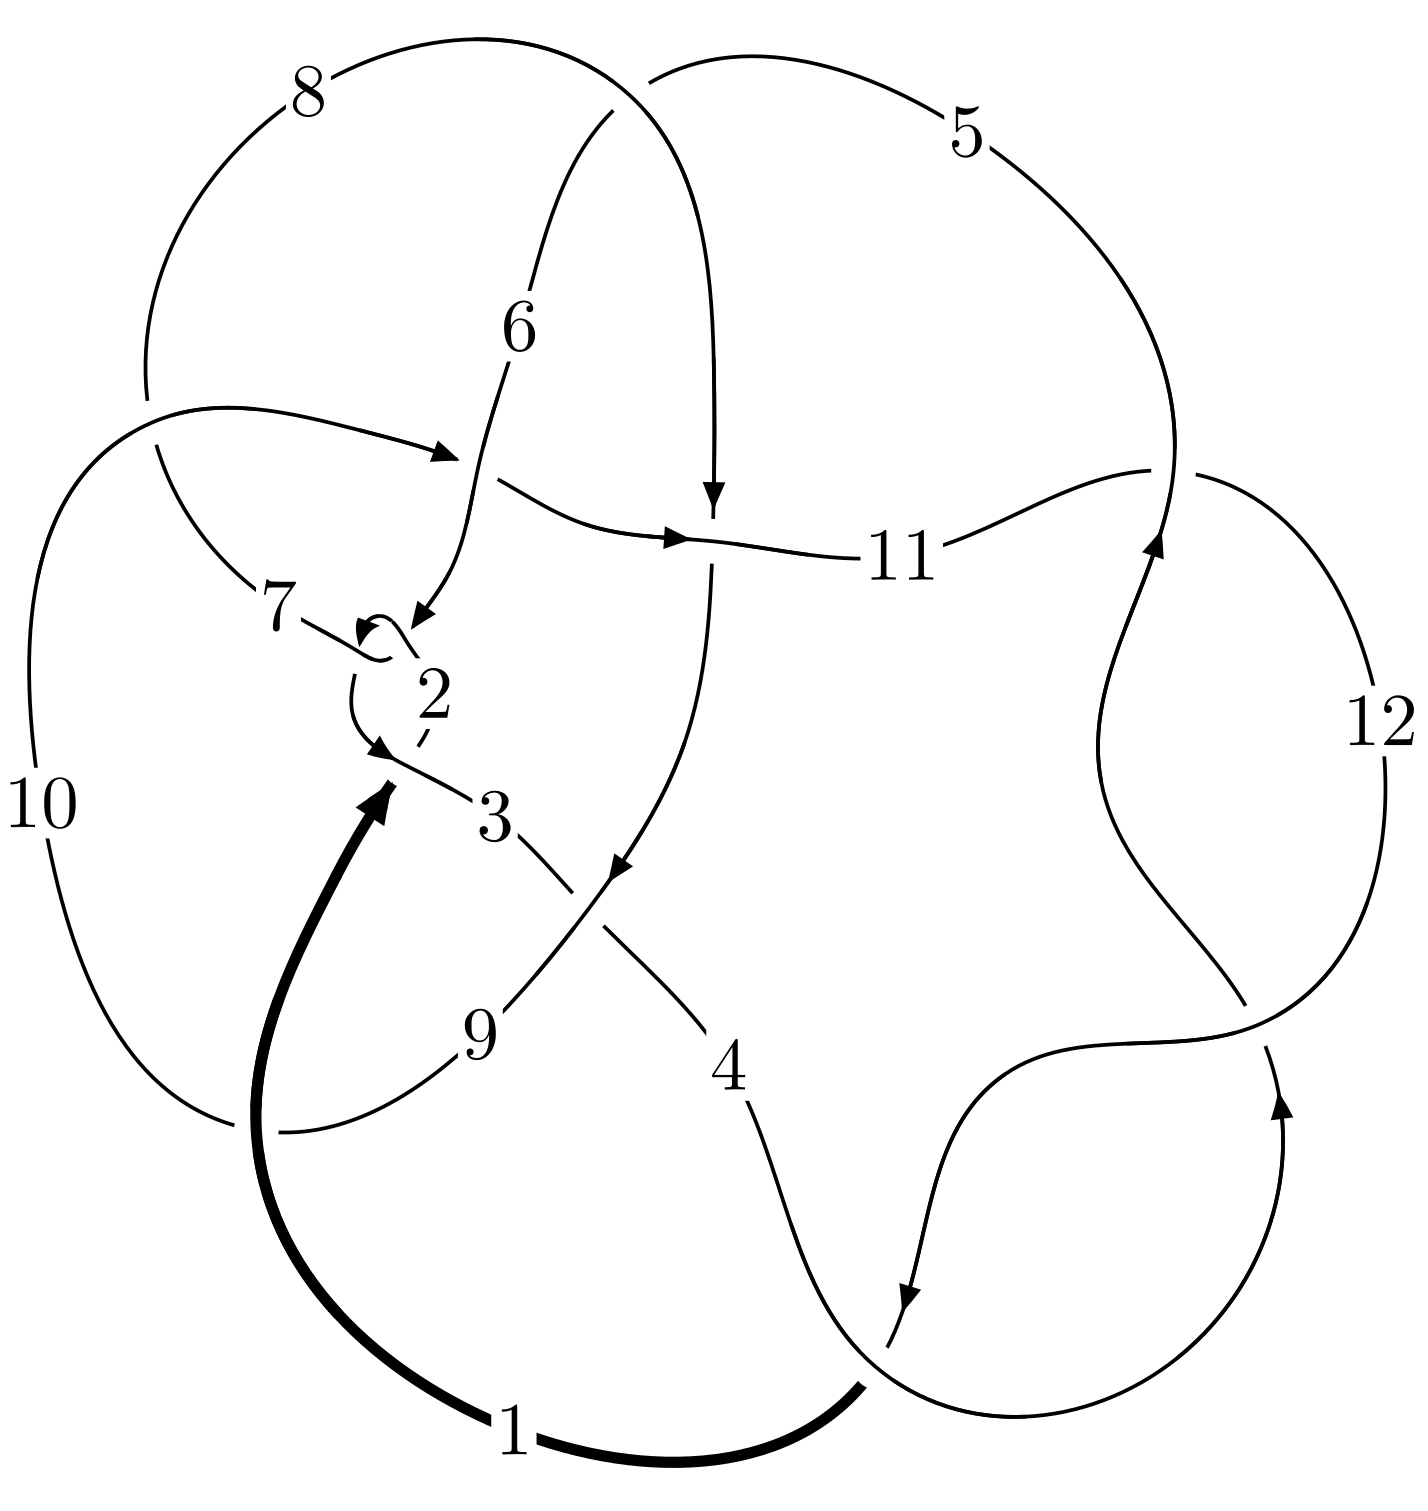
\includegraphics[width=112pt]{../../../GIT/diagram.site/Diagrams/png/1404_12a_0603.png}\\
\ \ \ A knot diagram\footnotemark}&
\allowdisplaybreaks
\textbf{Linearized knot diagam} \\
\cline{2-2}
 &
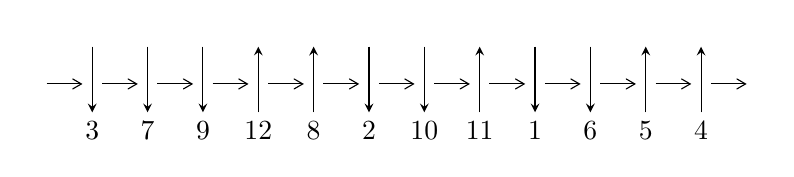
\begin{tikzpicture}[x=20pt, y=17pt]
	% nodes
	\node (C0) at (0, 0) {};
	\node (C1) at (1, 0) {};
	\node (C1U) at (1, +1) {};
	\node (C1D) at (1, -1) {3};

	\node (C2) at (2, 0) {};
	\node (C2U) at (2, +1) {};
	\node (C2D) at (2, -1) {7};

	\node (C3) at (3, 0) {};
	\node (C3U) at (3, +1) {};
	\node (C3D) at (3, -1) {9};

	\node (C4) at (4, 0) {};
	\node (C4U) at (4, +1) {};
	\node (C4D) at (4, -1) {12};

	\node (C5) at (5, 0) {};
	\node (C5U) at (5, +1) {};
	\node (C5D) at (5, -1) {8};

	\node (C6) at (6, 0) {};
	\node (C6U) at (6, +1) {};
	\node (C6D) at (6, -1) {2};

	\node (C7) at (7, 0) {};
	\node (C7U) at (7, +1) {};
	\node (C7D) at (7, -1) {10};

	\node (C8) at (8, 0) {};
	\node (C8U) at (8, +1) {};
	\node (C8D) at (8, -1) {11};

	\node (C9) at (9, 0) {};
	\node (C9U) at (9, +1) {};
	\node (C9D) at (9, -1) {1};

	\node (C10) at (10, 0) {};
	\node (C10U) at (10, +1) {};
	\node (C10D) at (10, -1) {6};

	\node (C11) at (11, 0) {};
	\node (C11U) at (11, +1) {};
	\node (C11D) at (11, -1) {5};

	\node (C12) at (12, 0) {};
	\node (C12U) at (12, +1) {};
	\node (C12D) at (12, -1) {4};
	\node (C13) at (13, 0) {};

	% arrows
	\draw[->,>={angle 60}]
	(C0) edge (C1) (C1) edge (C2) (C2) edge (C3) (C3) edge (C4) (C4) edge (C5) (C5) edge (C6) (C6) edge (C7) (C7) edge (C8) (C8) edge (C9) (C9) edge (C10) (C10) edge (C11) (C11) edge (C12) (C12) edge (C13) ;	\draw[->,>=stealth]
	(C1U) edge (C1D) (C2U) edge (C2D) (C3U) edge (C3D) (C4D) edge (C4U) (C5D) edge (C5U) (C6U) edge (C6D) (C7U) edge (C7D) (C8D) edge (C8U) (C9U) edge (C9D) (C10U) edge (C10D) (C11D) edge (C11U) (C12D) edge (C12U) ;
	\end{tikzpicture} \\
\hhline{~~} \\& 
\textbf{Solving Sequence} \\ \cline{2-2} 
 &
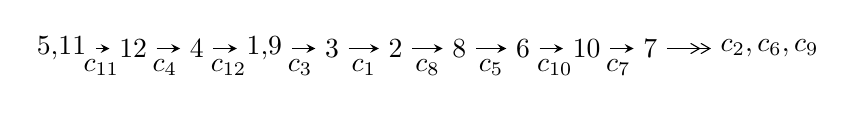
\begin{tikzpicture}[x=23pt, y=7pt]
	% node
	\node (A0) at (-1/8, 0) {5,11};
	\node (A1) at (1, 0) {12};
	\node (A2) at (2, 0) {4};
	\node (A3) at (49/16, 0) {1,9};
	\node (A4) at (33/8, 0) {3};
	\node (A5) at (41/8, 0) {2};
	\node (A6) at (49/8, 0) {8};
	\node (A7) at (57/8, 0) {6};
	\node (A8) at (65/8, 0) {10};
	\node (A9) at (73/8, 0) {7};
	\node (C1) at (1/2, -1) {$c_{11}$};
	\node (C2) at (3/2, -1) {$c_{4}$};
	\node (C3) at (5/2, -1) {$c_{12}$};
	\node (C4) at (29/8, -1) {$c_{3}$};
	\node (C5) at (37/8, -1) {$c_{1}$};
	\node (C6) at (45/8, -1) {$c_{8}$};
	\node (C7) at (53/8, -1) {$c_{5}$};
	\node (C8) at (61/8, -1) {$c_{10}$};
	\node (C9) at (69/8, -1) {$c_{7}$};
	\node (A10) at (11, 0) {$c_{2},c_{6},c_{9}$};

	% edge
	\draw[->,>=stealth]	
	(A0) edge (A1) (A1) edge (A2) (A2) edge (A3) (A3) edge (A4) (A4) edge (A5) (A5) edge (A6) (A6) edge (A7) (A7) edge (A8) (A8) edge (A9) ;
	\draw[->>,>={angle 60}]	
	(A9) edge (A10);
\end{tikzpicture} \\ 

\end{tabular} \\

\footnotetext{
The image of knot diagram is generated by the software ``\textbf{Draw programme}" developed by Andrew Bartholomew(\url{http://www.layer8.co.uk/maths/draw/index.htm\#Running-draw}), where we modified some parts for our purpose(\url{https://github.com/CATsTAILs/LinksPainter}).
}\phantom \\ \newline 
\centering \textbf{Ideals for irreducible components\footnotemark of $X_{\text{par}}$} 
 
\begin{align*}
I^u_{1}&=\langle 
-2.64474\times10^{364} u^{132}-1.02887\times10^{365} u^{131}+\cdots+2.92376\times10^{364} b-7.83824\times10^{364},\\
\phantom{I^u_{1}}&\phantom{= \langle  }1.91797\times10^{364} u^{132}+9.44885\times10^{364} u^{131}+\cdots+2.92376\times10^{364} a+1.78055\times10^{365},\\
\phantom{I^u_{1}}&\phantom{= \langle  }u^{133}+4 u^{132}+\cdots+18 u+1\rangle \\
I^u_{2}&=\langle 
-2338 u^{25}-12252 u^{24}+\cdots+18671 b-18146,\;-15486 u^{25}-29931 u^{24}+\cdots+18671 a+59714,\\
\phantom{I^u_{2}}&\phantom{= \langle  }u^{26}+u^{25}+\cdots-2 u+1\rangle \\
\\
\end{align*}
\raggedright * 2 irreducible components of $\dim_{\mathbb{C}}=0$, with total 159 representations.\\
\footnotetext{All coefficients of polynomials are rational numbers. But the coefficients are sometimes approximated in decimal forms when there is not enough margin.}
\newpage
\renewcommand{\arraystretch}{1}
\centering \section*{I. $I^u_{1}= \langle -2.64\times10^{364} u^{132}-1.03\times10^{365} u^{131}+\cdots+2.92\times10^{364} b-7.84\times10^{364},\;1.92\times10^{364} u^{132}+9.45\times10^{364} u^{131}+\cdots+2.92\times10^{364} a+1.78\times10^{365},\;u^{133}+4 u^{132}+\cdots+18 u+1 \rangle$}
\flushleft \textbf{(i) Arc colorings}\\
\begin{tabular}{m{7pt} m{180pt} m{7pt} m{180pt} }
\flushright $a_{5}=$&$\begin{pmatrix}0\\u\end{pmatrix}$ \\
\flushright $a_{11}=$&$\begin{pmatrix}1\\0\end{pmatrix}$ \\
\flushright $a_{12}=$&$\begin{pmatrix}1\\- u^2\end{pmatrix}$ \\
\flushright $a_{4}=$&$\begin{pmatrix}- u\\u^3+u\end{pmatrix}$ \\
\flushright $a_{1}=$&$\begin{pmatrix}u^2+1\\- u^4-2 u^2\end{pmatrix}$ \\
\flushright $a_{9}=$&$\begin{pmatrix}-0.655993 u^{132}-3.23175 u^{131}+\cdots-268.477 u-6.08993\\0.904567 u^{132}+3.51901 u^{131}+\cdots+27.3508 u+2.68088\end{pmatrix}$ \\
\flushright $a_{3}=$&$\begin{pmatrix}2.36500 u^{132}+9.81964 u^{131}+\cdots+400.736 u+24.4482\\0.861748 u^{132}+3.26370 u^{131}+\cdots+63.9327 u+2.76443\end{pmatrix}$ \\
\flushright $a_{2}=$&$\begin{pmatrix}0.500905 u^{132}+1.14522 u^{131}+\cdots-19.0597 u-10.5361\\-0.0621254 u^{132}+0.252358 u^{131}+\cdots+7.15415 u-1.03549\end{pmatrix}$ \\
\flushright $a_{8}=$&$\begin{pmatrix}-1.56056 u^{132}-6.75076 u^{131}+\cdots-295.828 u-8.77081\\0.904567 u^{132}+3.51901 u^{131}+\cdots+27.3508 u+2.68088\end{pmatrix}$ \\
\flushright $a_{6}=$&$\begin{pmatrix}2.44617 u^{132}+10.3270 u^{131}+\cdots+319.714 u+20.7248\\-0.378624 u^{132}-1.55141 u^{131}+\cdots+16.1274 u+0.732186\end{pmatrix}$ \\
\flushright $a_{10}=$&$\begin{pmatrix}-1.24955 u^{132}-5.63197 u^{131}+\cdots-317.747 u-10.0100\\0.639277 u^{132}+2.53166 u^{131}+\cdots+21.4354 u+2.42305\end{pmatrix}$ \\
\flushright $a_{7}=$&$\begin{pmatrix}-1.11577 u^{132}-4.52867 u^{131}+\cdots-100.102 u+6.85622\\-0.267124 u^{132}-0.836064 u^{131}+\cdots+47.1787 u+4.78908\end{pmatrix}$\\&\end{tabular}
\flushleft \textbf{(ii) Obstruction class $= -1$}\\~\\
\flushleft \textbf{(iii) Cusp Shapes $= -9.94811 u^{132}-38.2270 u^{131}+\cdots-105.374 u+7.68191$}\\~\\
\newpage\renewcommand{\arraystretch}{1}
\flushleft \textbf{(iv) u-Polynomials at the component}\newline \\
\begin{tabular}{m{50pt}|m{274pt}}
Crossings & \hspace{64pt}u-Polynomials at each crossing \\
\hline $$\begin{aligned}c_{1}\end{aligned}$$&$\begin{aligned}
&u^{133}+52 u^{132}+\cdots+48754 u+1849
\end{aligned}$\\
\hline $$\begin{aligned}c_{2},c_{6}\end{aligned}$$&$\begin{aligned}
&u^{133}-26 u^{131}+\cdots+54 u+43
\end{aligned}$\\
\hline $$\begin{aligned}c_{3}\end{aligned}$$&$\begin{aligned}
&u^{133}-2 u^{132}+\cdots+11980 u+919
\end{aligned}$\\
\hline $$\begin{aligned}c_{4},c_{11},c_{12}\end{aligned}$$&$\begin{aligned}
&u^{133}+4 u^{132}+\cdots+18 u+1
\end{aligned}$\\
\hline $$\begin{aligned}c_{5}\end{aligned}$$&$\begin{aligned}
&u^{133}+11 u^{132}+\cdots+114108 u+20779
\end{aligned}$\\
\hline $$\begin{aligned}c_{7}\end{aligned}$$&$\begin{aligned}
&u^{133}+12 u^{132}+\cdots-10013 u+1819
\end{aligned}$\\
\hline $$\begin{aligned}c_{8}\end{aligned}$$&$\begin{aligned}
&u^{133}-8 u^{132}+\cdots+4740 u+2736
\end{aligned}$\\
\hline $$\begin{aligned}c_{9}\end{aligned}$$&$\begin{aligned}
&u^{133}+3 u^{132}+\cdots+42284 u-2231
\end{aligned}$\\
\hline $$\begin{aligned}c_{10}\end{aligned}$$&$\begin{aligned}
&u^{133}+u^{132}+\cdots+22010 u-1007
\end{aligned}$\\
\hline
\end{tabular}\\~\\
\newpage\renewcommand{\arraystretch}{1}
\flushleft \textbf{(v) Riley Polynomials at the component}\newline \\
\begin{tabular}{m{50pt}|m{274pt}}
Crossings & \hspace{64pt}Riley Polynomials at each crossing \\
\hline $$\begin{aligned}c_{1}\end{aligned}$$&$\begin{aligned}
&y^{133}+64 y^{132}+\cdots-347471326 y-3418801
\end{aligned}$\\
\hline $$\begin{aligned}c_{2},c_{6}\end{aligned}$$&$\begin{aligned}
&y^{133}-52 y^{132}+\cdots+48754 y-1849
\end{aligned}$\\
\hline $$\begin{aligned}c_{3}\end{aligned}$$&$\begin{aligned}
&y^{133}-16 y^{132}+\cdots+28417488 y-844561
\end{aligned}$\\
\hline $$\begin{aligned}c_{4},c_{11},c_{12}\end{aligned}$$&$\begin{aligned}
&y^{133}+144 y^{132}+\cdots-178 y-1
\end{aligned}$\\
\hline $$\begin{aligned}c_{5}\end{aligned}$$&$\begin{aligned}
&y^{133}+37 y^{132}+\cdots-27554143614 y-431766841
\end{aligned}$\\
\hline $$\begin{aligned}c_{7}\end{aligned}$$&$\begin{aligned}
&y^{133}+2 y^{132}+\cdots+17932229 y-3308761
\end{aligned}$\\
\hline $$\begin{aligned}c_{8}\end{aligned}$$&$\begin{aligned}
&y^{133}+26 y^{132}+\cdots-64564560 y-7485696
\end{aligned}$\\
\hline $$\begin{aligned}c_{9}\end{aligned}$$&$\begin{aligned}
&y^{133}-25 y^{132}+\cdots+651416174 y-4977361
\end{aligned}$\\
\hline $$\begin{aligned}c_{10}\end{aligned}$$&$\begin{aligned}
&y^{133}+35 y^{132}+\cdots+25824104 y-1014049
\end{aligned}$\\
\hline
\end{tabular}\\~\\
\newpage\flushleft \textbf{(vi) Complex Volumes and Cusp Shapes}
$$\begin{array}{c|c|c}  
\text{Solutions to }I^u_{1}& \I (\text{vol} + \sqrt{-1}CS) & \text{Cusp shape}\\
 \hline 
\begin{aligned}
u &= -0.317390 + 0.951720 I \\
a &= \phantom{-}1.48827 - 0.25479 I \\
b &= \phantom{-}0.757216 + 0.344540 I\end{aligned}
 & -0.13837 - 1.80283 I & \phantom{-0.000000 } 0 \\ \hline\begin{aligned}
u &= -0.317390 - 0.951720 I \\
a &= \phantom{-}1.48827 + 0.25479 I \\
b &= \phantom{-}0.757216 - 0.344540 I\end{aligned}
 & -0.13837 + 1.80283 I & \phantom{-0.000000 } 0 \\ \hline\begin{aligned}
u &= \phantom{-}0.000414 + 1.006760 I \\
a &= \phantom{-}0.907735 - 0.505915 I \\
b &= \phantom{-}0.454679 - 0.046619 I\end{aligned}
 & -0.85528 + 1.37756 I & \phantom{-0.000000 } 0 \\ \hline\begin{aligned}
u &= \phantom{-}0.000414 - 1.006760 I \\
a &= \phantom{-}0.907735 + 0.505915 I \\
b &= \phantom{-}0.454679 + 0.046619 I\end{aligned}
 & -0.85528 - 1.37756 I & \phantom{-0.000000 } 0 \\ \hline\begin{aligned}
u &= \phantom{-}0.369042 + 0.904093 I \\
a &= \phantom{-}1.49938 + 0.10474 I \\
b &= \phantom{-}0.699547 - 0.487167 I\end{aligned}
 & -0.32005 - 2.62744 I & \phantom{-0.000000 } 0 \\ \hline\begin{aligned}
u &= \phantom{-}0.369042 - 0.904093 I \\
a &= \phantom{-}1.49938 - 0.10474 I \\
b &= \phantom{-}0.699547 + 0.487167 I\end{aligned}
 & -0.32005 + 2.62744 I & \phantom{-0.000000 } 0 \\ \hline\begin{aligned}
u &= -0.803088 + 0.636718 I \\
a &= \phantom{-}0.484658 + 0.531000 I \\
b &= -0.775385 + 0.851791 I\end{aligned}
 & -4.78432 - 7.01607 I & \phantom{-0.000000 } 0 \\ \hline\begin{aligned}
u &= -0.803088 - 0.636718 I \\
a &= \phantom{-}0.484658 - 0.531000 I \\
b &= -0.775385 - 0.851791 I\end{aligned}
 & -4.78432 + 7.01607 I & \phantom{-0.000000 } 0 \\ \hline\begin{aligned}
u &= -0.793242 + 0.649364 I \\
a &= \phantom{-}0.316921 + 0.646051 I \\
b &= -1.028850 + 0.950405 I\end{aligned}
 & \phantom{-}0.6941 - 14.9364 I & \phantom{-0.000000 } 0 \\ \hline\begin{aligned}
u &= -0.793242 - 0.649364 I \\
a &= \phantom{-}0.316921 - 0.646051 I \\
b &= -1.028850 - 0.950405 I\end{aligned}
 & \phantom{-}0.6941 + 14.9364 I & \phantom{-0.000000 } 0\\
 \hline 
 \end{array}$$\newpage$$\begin{array}{c|c|c}  
\text{Solutions to }I^u_{1}& \I (\text{vol} + \sqrt{-1}CS) & \text{Cusp shape}\\
 \hline 
\begin{aligned}
u &= \phantom{-}0.793523 + 0.655020 I \\
a &= \phantom{-}0.311114 - 0.584099 I \\
b &= -1.019840 - 0.865635 I\end{aligned}
 & \phantom{-}2.41217 + 8.91087 I & \phantom{-0.000000 } 0 \\ \hline\begin{aligned}
u &= \phantom{-}0.793523 - 0.655020 I \\
a &= \phantom{-}0.311114 + 0.584099 I \\
b &= -1.019840 + 0.865635 I\end{aligned}
 & \phantom{-}2.41217 - 8.91087 I & \phantom{-0.000000 } 0 \\ \hline\begin{aligned}
u &= -0.935358 + 0.435263 I \\
a &= -0.330740 + 0.419531 I \\
b &= -0.631739 - 0.591068 I\end{aligned}
 & \phantom{-}1.37484 + 9.33049 I & \phantom{-0.000000 } 0 \\ \hline\begin{aligned}
u &= -0.935358 - 0.435263 I \\
a &= -0.330740 - 0.419531 I \\
b &= -0.631739 + 0.591068 I\end{aligned}
 & \phantom{-}1.37484 - 9.33049 I & \phantom{-0.000000 } 0 \\ \hline\begin{aligned}
u &= \phantom{-}0.956015 + 0.391472 I \\
a &= -0.180667 - 0.451075 I \\
b &= -0.595131 + 0.477995 I\end{aligned}
 & \phantom{-}3.19901 - 3.27930 I & \phantom{-0.000000 } 0 \\ \hline\begin{aligned}
u &= \phantom{-}0.956015 - 0.391472 I \\
a &= -0.180667 + 0.451075 I \\
b &= -0.595131 - 0.477995 I\end{aligned}
 & \phantom{-}3.19901 + 3.27930 I & \phantom{-0.000000 } 0 \\ \hline\begin{aligned}
u &= \phantom{-}0.498790 + 0.934638 I \\
a &= \phantom{-}0.322872 - 0.250760 I \\
b &= -1.020790 - 0.209680 I\end{aligned}
 & \phantom{-}1.84987 + 2.34571 I & \phantom{-0.000000 } 0 \\ \hline\begin{aligned}
u &= \phantom{-}0.498790 - 0.934638 I \\
a &= \phantom{-}0.322872 + 0.250760 I \\
b &= -1.020790 + 0.209680 I\end{aligned}
 & \phantom{-}1.84987 - 2.34571 I & \phantom{-0.000000 } 0 \\ \hline\begin{aligned}
u &= -0.789480 + 0.492341 I \\
a &= -0.242498 - 0.247167 I \\
b &= \phantom{-}0.227250 - 0.984213 I\end{aligned}
 & -2.11830 - 6.37096 I & \phantom{-0.000000 } 0 \\ \hline\begin{aligned}
u &= -0.789480 - 0.492341 I \\
a &= -0.242498 + 0.247167 I \\
b &= \phantom{-}0.227250 + 0.984213 I\end{aligned}
 & -2.11830 + 6.37096 I & \phantom{-0.000000 } 0\\
 \hline 
 \end{array}$$\newpage$$\begin{array}{c|c|c}  
\text{Solutions to }I^u_{1}& \I (\text{vol} + \sqrt{-1}CS) & \text{Cusp shape}\\
 \hline 
\begin{aligned}
u &= \phantom{-}0.932967 + 0.567128 I \\
a &= \phantom{-}0.453567 - 0.242141 I \\
b &= -0.685684 - 0.500427 I\end{aligned}
 & \phantom{-}0.94295 + 3.39839 I & \phantom{-0.000000 } 0 \\ \hline\begin{aligned}
u &= \phantom{-}0.932967 - 0.567128 I \\
a &= \phantom{-}0.453567 + 0.242141 I \\
b &= -0.685684 + 0.500427 I\end{aligned}
 & \phantom{-}0.94295 - 3.39839 I & \phantom{-0.000000 } 0 \\ \hline\begin{aligned}
u &= \phantom{-}0.658045 + 0.586349 I \\
a &= -0.036517 + 0.301429 I \\
b &= \phantom{-}0.413199 + 0.649549 I\end{aligned}
 & -0.02575 + 2.01548 I & \phantom{-0.000000 } 0 \\ \hline\begin{aligned}
u &= \phantom{-}0.658045 - 0.586349 I \\
a &= -0.036517 - 0.301429 I \\
b &= \phantom{-}0.413199 - 0.649549 I\end{aligned}
 & -0.02575 - 2.01548 I & \phantom{-0.000000 } 0 \\ \hline\begin{aligned}
u &= -0.958383 + 0.586194 I \\
a &= -0.189165 + 0.040884 I \\
b &= -0.175318 - 0.636952 I\end{aligned}
 & -4.36490 + 1.21700 I & \phantom{-0.000000 } 0 \\ \hline\begin{aligned}
u &= -0.958383 - 0.586194 I \\
a &= -0.189165 - 0.040884 I \\
b &= -0.175318 + 0.636952 I\end{aligned}
 & -4.36490 - 1.21700 I & \phantom{-0.000000 } 0 \\ \hline\begin{aligned}
u &= -0.426635 + 0.754500 I \\
a &= \phantom{-}0.265362 + 0.064534 I \\
b &= -1.151620 + 0.038490 I\end{aligned}
 & \phantom{-}0.72377 + 3.99082 I & \phantom{-0.000000 } 0 \\ \hline\begin{aligned}
u &= -0.426635 - 0.754500 I \\
a &= \phantom{-}0.265362 - 0.064534 I \\
b &= -1.151620 - 0.038490 I\end{aligned}
 & \phantom{-}0.72377 - 3.99082 I & \phantom{-0.000000 } 0 \\ \hline\begin{aligned}
u &= -0.672366 + 0.529127 I \\
a &= \phantom{-}0.851817 + 0.281364 I \\
b &= -0.266858 + 0.657749 I\end{aligned}
 & -2.44476 + 1.49394 I & \phantom{-0.000000 } 0 \\ \hline\begin{aligned}
u &= -0.672366 - 0.529127 I \\
a &= \phantom{-}0.851817 - 0.281364 I \\
b &= -0.266858 - 0.657749 I\end{aligned}
 & -2.44476 - 1.49394 I & \phantom{-0.000000 } 0\\
 \hline 
 \end{array}$$\newpage$$\begin{array}{c|c|c}  
\text{Solutions to }I^u_{1}& \I (\text{vol} + \sqrt{-1}CS) & \text{Cusp shape}\\
 \hline 
\begin{aligned}
u &= \phantom{-}0.407366 + 0.705544 I \\
a &= \phantom{-}1.237480 - 0.100857 I \\
b &= \phantom{-}0.317154 - 0.559779 I\end{aligned}
 & -1.33061 + 1.48114 I & \phantom{-0.000000 } 0 \\ \hline\begin{aligned}
u &= \phantom{-}0.407366 - 0.705544 I \\
a &= \phantom{-}1.237480 + 0.100857 I \\
b &= \phantom{-}0.317154 + 0.559779 I\end{aligned}
 & -1.33061 - 1.48114 I & \phantom{-0.000000 } 0 \\ \hline\begin{aligned}
u &= \phantom{-}0.106132 + 1.212180 I \\
a &= \phantom{-}0.540451 - 0.882730 I \\
b &= \phantom{-}0.227641 - 0.264956 I\end{aligned}
 & -0.91739 + 1.45459 I & \phantom{-0.000000 } 0 \\ \hline\begin{aligned}
u &= \phantom{-}0.106132 - 1.212180 I \\
a &= \phantom{-}0.540451 + 0.882730 I \\
b &= \phantom{-}0.227641 + 0.264956 I\end{aligned}
 & -0.91739 - 1.45459 I & \phantom{-0.000000 } 0 \\ \hline\begin{aligned}
u &= \phantom{-}0.649189 + 0.390265 I \\
a &= -0.292317 + 0.359202 I \\
b &= \phantom{-}0.660502 + 0.993791 I\end{aligned}
 & -0.25396 + 2.43752 I & \phantom{-0.000000 } 0 \\ \hline\begin{aligned}
u &= \phantom{-}0.649189 - 0.390265 I \\
a &= -0.292317 - 0.359202 I \\
b &= \phantom{-}0.660502 - 0.993791 I\end{aligned}
 & -0.25396 - 2.43752 I & \phantom{-0.000000 } 0 \\ \hline\begin{aligned}
u &= \phantom{-}0.506366 + 0.515867 I \\
a &= -0.026354 + 1.228440 I \\
b &= \phantom{-}1.108190 + 0.793659 I\end{aligned}
 & \phantom{-}2.75321 + 1.11683 I & \phantom{-0.000000 } 0 \\ \hline\begin{aligned}
u &= \phantom{-}0.506366 - 0.515867 I \\
a &= -0.026354 - 1.228440 I \\
b &= \phantom{-}1.108190 - 0.793659 I\end{aligned}
 & \phantom{-}2.75321 - 1.11683 I & \phantom{-0.000000 } 0 \\ \hline\begin{aligned}
u &= -0.481846 + 0.531634 I \\
a &= -0.20249 - 1.40276 I \\
b &= \phantom{-}1.09151 - 0.94036 I\end{aligned}
 & \phantom{-}2.44358 - 6.00898 I & \phantom{-0.000000 } 0 \\ \hline\begin{aligned}
u &= -0.481846 - 0.531634 I \\
a &= -0.20249 + 1.40276 I \\
b &= \phantom{-}1.09151 + 0.94036 I\end{aligned}
 & \phantom{-}2.44358 + 6.00898 I & \phantom{-0.000000 } 0\\
 \hline 
 \end{array}$$\newpage$$\begin{array}{c|c|c}  
\text{Solutions to }I^u_{1}& \I (\text{vol} + \sqrt{-1}CS) & \text{Cusp shape}\\
 \hline 
\begin{aligned}
u &= \phantom{-}0.656088 + 0.255849 I \\
a &= \phantom{-}0.52898 - 1.37981 I \\
b &= -0.681640 + 0.041539 I\end{aligned}
 & \phantom{-}3.76926 + 1.77877 I & \phantom{-0.000000 } 0 \\ \hline\begin{aligned}
u &= \phantom{-}0.656088 - 0.255849 I \\
a &= \phantom{-}0.52898 + 1.37981 I \\
b &= -0.681640 - 0.041539 I\end{aligned}
 & \phantom{-}3.76926 - 1.77877 I & \phantom{-0.000000 } 0 \\ \hline\begin{aligned}
u &= \phantom{-}0.024261 + 1.300360 I \\
a &= \phantom{-}0.80241 + 1.25166 I \\
b &= \phantom{-}0.392384 + 0.629169 I\end{aligned}
 & -1.84210 + 3.58791 I & \phantom{-0.000000 } 0 \\ \hline\begin{aligned}
u &= \phantom{-}0.024261 - 1.300360 I \\
a &= \phantom{-}0.80241 - 1.25166 I \\
b &= \phantom{-}0.392384 - 0.629169 I\end{aligned}
 & -1.84210 - 3.58791 I & \phantom{-0.000000 } 0 \\ \hline\begin{aligned}
u &= \phantom{-}0.634032 + 0.204038 I \\
a &= -0.266567 + 0.023162 I \\
b &= \phantom{-}0.96643 + 1.09114 I\end{aligned}
 & \phantom{-}1.81642 + 6.34178 I & \phantom{-0.000000 } 0 \\ \hline\begin{aligned}
u &= \phantom{-}0.634032 - 0.204038 I \\
a &= -0.266567 - 0.023162 I \\
b &= \phantom{-}0.96643 - 1.09114 I\end{aligned}
 & \phantom{-}1.81642 - 6.34178 I & \phantom{-0.000000 } 0 \\ \hline\begin{aligned}
u &= -0.591817 + 0.305159 I \\
a &= \phantom{-}0.47167 + 1.82209 I \\
b &= -0.722007 + 0.064641 I\end{aligned}
 & \phantom{-}2.08204 - 7.64852 I & \phantom{-0.000000 } 0 \\ \hline\begin{aligned}
u &= -0.591817 - 0.305159 I \\
a &= \phantom{-}0.47167 - 1.82209 I \\
b &= -0.722007 - 0.064641 I\end{aligned}
 & \phantom{-}2.08204 + 7.64852 I & \phantom{-0.000000 } 0 \\ \hline\begin{aligned}
u &= -0.115208 + 1.393630 I \\
a &= \phantom{-}0.36616 + 1.69593 I \\
b &= -0.175512 + 0.385658 I\end{aligned}
 & -7.28259 - 1.99857 I & \phantom{-0.000000 } 0 \\ \hline\begin{aligned}
u &= -0.115208 - 1.393630 I \\
a &= \phantom{-}0.36616 - 1.69593 I \\
b &= -0.175512 - 0.385658 I\end{aligned}
 & -7.28259 + 1.99857 I & \phantom{-0.000000 } 0\\
 \hline 
 \end{array}$$\newpage$$\begin{array}{c|c|c}  
\text{Solutions to }I^u_{1}& \I (\text{vol} + \sqrt{-1}CS) & \text{Cusp shape}\\
 \hline 
\begin{aligned}
u &= -0.576843 + 0.161115 I \\
a &= -0.352819 + 0.183120 I \\
b &= \phantom{-}1.02384 - 0.98527 I\end{aligned}
 & \phantom{-}2.25476 - 1.57690 I & \phantom{-0.000000 } 0 \\ \hline\begin{aligned}
u &= -0.576843 - 0.161115 I \\
a &= -0.352819 - 0.183120 I \\
b &= \phantom{-}1.02384 + 0.98527 I\end{aligned}
 & \phantom{-}2.25476 + 1.57690 I & \phantom{-0.000000 } 0 \\ \hline\begin{aligned}
u &= \phantom{-}0.157819 + 1.404700 I \\
a &= \phantom{-}0.38426 + 2.21112 I \\
b &= \phantom{-}1.16806 + 1.82923 I\end{aligned}
 & -3.28021 + 9.03412 I & \phantom{-0.000000 } 0 \\ \hline\begin{aligned}
u &= \phantom{-}0.157819 - 1.404700 I \\
a &= \phantom{-}0.38426 - 2.21112 I \\
b &= \phantom{-}1.16806 - 1.82923 I\end{aligned}
 & -3.28021 - 9.03412 I & \phantom{-0.000000 } 0 \\ \hline\begin{aligned}
u &= -0.129646 + 1.407920 I \\
a &= \phantom{-}0.52271 - 2.11793 I \\
b &= \phantom{-}1.31501 - 1.72724 I\end{aligned}
 & -2.74273 - 3.87928 I & \phantom{-0.000000 } 0 \\ \hline\begin{aligned}
u &= -0.129646 - 1.407920 I \\
a &= \phantom{-}0.52271 + 2.11793 I \\
b &= \phantom{-}1.31501 + 1.72724 I\end{aligned}
 & -2.74273 + 3.87928 I & \phantom{-0.000000 } 0 \\ \hline\begin{aligned}
u &= -0.00898 + 1.41834 I \\
a &= \phantom{-}0.869029 - 0.280038 I \\
b &= \phantom{-}1.89525 - 0.21062 I\end{aligned}
 & -1.87843 - 2.86423 I & \phantom{-0.000000 } 0 \\ \hline\begin{aligned}
u &= -0.00898 - 1.41834 I \\
a &= \phantom{-}0.869029 + 0.280038 I \\
b &= \phantom{-}1.89525 + 0.21062 I\end{aligned}
 & -1.87843 + 2.86423 I & \phantom{-0.000000 } 0 \\ \hline\begin{aligned}
u &= \phantom{-}0.425893 + 0.388958 I \\
a &= \phantom{-}0.749508 + 0.920587 I \\
b &= \phantom{-}1.090570 - 0.092383 I\end{aligned}
 & \phantom{-}3.04373 + 2.24122 I & \phantom{-0.000000 } 0 \\ \hline\begin{aligned}
u &= \phantom{-}0.425893 - 0.388958 I \\
a &= \phantom{-}0.749508 - 0.920587 I \\
b &= \phantom{-}1.090570 + 0.092383 I\end{aligned}
 & \phantom{-}3.04373 - 2.24122 I & \phantom{-0.000000 } 0\\
 \hline 
 \end{array}$$\newpage$$\begin{array}{c|c|c}  
\text{Solutions to }I^u_{1}& \I (\text{vol} + \sqrt{-1}CS) & \text{Cusp shape}\\
 \hline 
\begin{aligned}
u &= \phantom{-}0.17101 + 1.41706 I \\
a &= -0.19054 - 1.45824 I \\
b &= -0.198228 - 0.320181 I\end{aligned}
 & -1.56608 + 4.61751 I & \phantom{-0.000000 } 0 \\ \hline\begin{aligned}
u &= \phantom{-}0.17101 - 1.41706 I \\
a &= -0.19054 + 1.45824 I \\
b &= -0.198228 + 0.320181 I\end{aligned}
 & -1.56608 - 4.61751 I & \phantom{-0.000000 } 0 \\ \hline\begin{aligned}
u &= -0.16050 + 1.44536 I \\
a &= -0.35715 + 1.61866 I \\
b &= -0.235486 + 0.363547 I\end{aligned}
 & -3.57964 - 10.24340 I & \phantom{-0.000000 } 0 \\ \hline\begin{aligned}
u &= -0.16050 - 1.44536 I \\
a &= -0.35715 - 1.61866 I \\
b &= -0.235486 - 0.363547 I\end{aligned}
 & -3.57964 + 10.24340 I & \phantom{-0.000000 } 0 \\ \hline\begin{aligned}
u &= -0.168418 + 0.494494 I \\
a &= \phantom{-}0.674329 - 0.621285 I \\
b &= -0.789301 - 0.837924 I\end{aligned}
 & -4.60689 - 1.43800 I & -13.8922 + 4.9797 I \\ \hline\begin{aligned}
u &= -0.168418 - 0.494494 I \\
a &= \phantom{-}0.674329 + 0.621285 I \\
b &= -0.789301 + 0.837924 I\end{aligned}
 & -4.60689 + 1.43800 I & -13.8922 - 4.9797 I \\ \hline\begin{aligned}
u &= -0.06341 + 1.47689 I \\
a &= \phantom{-}0.08778 - 1.68631 I \\
b &= \phantom{-}1.04337 - 1.10273 I\end{aligned}
 & -5.88104 - 3.96728 I & \phantom{-0.000000 } 0 \\ \hline\begin{aligned}
u &= -0.06341 - 1.47689 I \\
a &= \phantom{-}0.08778 + 1.68631 I \\
b &= \phantom{-}1.04337 + 1.10273 I\end{aligned}
 & -5.88104 + 3.96728 I & \phantom{-0.000000 } 0 \\ \hline\begin{aligned}
u &= \phantom{-}0.01989 + 1.48051 I \\
a &= -0.49414 + 1.42885 I \\
b &= \phantom{-}0.790106 + 0.712369 I\end{aligned}
 & -9.73015 + 0.95948 I & \phantom{-0.000000 } 0 \\ \hline\begin{aligned}
u &= \phantom{-}0.01989 - 1.48051 I \\
a &= -0.49414 - 1.42885 I \\
b &= \phantom{-}0.790106 - 0.712369 I\end{aligned}
 & -9.73015 - 0.95948 I & \phantom{-0.000000 } 0\\
 \hline 
 \end{array}$$\newpage$$\begin{array}{c|c|c}  
\text{Solutions to }I^u_{1}& \I (\text{vol} + \sqrt{-1}CS) & \text{Cusp shape}\\
 \hline 
\begin{aligned}
u &= -0.043249 + 0.511103 I \\
a &= \phantom{-}1.214090 + 0.126404 I \\
b &= \phantom{-}0.109302 + 0.541830 I\end{aligned}
 & -0.583972 + 1.101550 I & -4.23096 - 5.60583 I \\ \hline\begin{aligned}
u &= -0.043249 - 0.511103 I \\
a &= \phantom{-}1.214090 - 0.126404 I \\
b &= \phantom{-}0.109302 - 0.541830 I\end{aligned}
 & -0.583972 - 1.101550 I & -4.23096 + 5.60583 I \\ \hline\begin{aligned}
u &= \phantom{-}0.133560 + 0.491181 I \\
a &= -1.90389 + 2.49784 I \\
b &= \phantom{-}0.372651 + 1.063630 I\end{aligned}
 & -1.26012 + 7.38742 I & -9.26674 - 9.57442 I \\ \hline\begin{aligned}
u &= \phantom{-}0.133560 - 0.491181 I \\
a &= -1.90389 - 2.49784 I \\
b &= \phantom{-}0.372651 - 1.063630 I\end{aligned}
 & -1.26012 - 7.38742 I & -9.26674 + 9.57442 I \\ \hline\begin{aligned}
u &= \phantom{-}0.04176 + 1.49067 I \\
a &= -0.47373 + 2.05790 I \\
b &= -0.89918 + 1.88657 I\end{aligned}
 & -5.92601 + 2.68412 I & \phantom{-0.000000 } 0 \\ \hline\begin{aligned}
u &= \phantom{-}0.04176 - 1.49067 I \\
a &= -0.47373 - 2.05790 I \\
b &= -0.89918 - 1.88657 I\end{aligned}
 & -5.92601 - 2.68412 I & \phantom{-0.000000 } 0 \\ \hline\begin{aligned}
u &= -0.04847 + 1.49413 I \\
a &= -0.78279 - 2.21960 I \\
b &= -1.18996 - 2.09454 I\end{aligned}
 & -7.06887 - 8.05152 I & \phantom{-0.000000 } 0 \\ \hline\begin{aligned}
u &= -0.04847 - 1.49413 I \\
a &= -0.78279 + 2.21960 I \\
b &= -1.18996 + 2.09454 I\end{aligned}
 & -7.06887 + 8.05152 I & \phantom{-0.000000 } 0 \\ \hline\begin{aligned}
u &= -0.285640 + 0.411254 I \\
a &= -1.67724 - 1.34413 I \\
b &= \phantom{-}0.674173 - 0.951931 I\end{aligned}
 & \phantom{-}0.21801 - 2.84449 I & -6.69111 + 5.42023 I \\ \hline\begin{aligned}
u &= -0.285640 - 0.411254 I \\
a &= -1.67724 + 1.34413 I \\
b &= \phantom{-}0.674173 + 0.951931 I\end{aligned}
 & \phantom{-}0.21801 + 2.84449 I & -6.69111 - 5.42023 I\\
 \hline 
 \end{array}$$\newpage$$\begin{array}{c|c|c}  
\text{Solutions to }I^u_{1}& \I (\text{vol} + \sqrt{-1}CS) & \text{Cusp shape}\\
 \hline 
\begin{aligned}
u &= -0.00411 + 1.49940 I \\
a &= -0.034013 + 1.247090 I \\
b &= -0.654002 + 1.001360 I\end{aligned}
 & -7.13066 + 0.99619 I & \phantom{-0.000000 } 0 \\ \hline\begin{aligned}
u &= -0.00411 - 1.49940 I \\
a &= -0.034013 - 1.247090 I \\
b &= -0.654002 - 1.001360 I\end{aligned}
 & -7.13066 - 0.99619 I & \phantom{-0.000000 } 0 \\ \hline\begin{aligned}
u &= -0.493767\phantom{ +0.000000I} \\
a &= \phantom{-}2.39133\phantom{ +0.000000I} \\
b &= -0.433102\phantom{ +0.000000I}\end{aligned}
 & -2.78828\phantom{ +0.000000I} & \phantom{-}7.19090\phantom{ +0.000000I} \\ \hline\begin{aligned}
u &= \phantom{-}0.18593 + 1.49544 I \\
a &= \phantom{-}0.23693 + 1.86590 I \\
b &= \phantom{-}0.87674 + 1.52250 I\end{aligned}
 & -6.47122 + 5.38417 I & \phantom{-0.000000 } 0 \\ \hline\begin{aligned}
u &= \phantom{-}0.18593 - 1.49544 I \\
a &= \phantom{-}0.23693 - 1.86590 I \\
b &= \phantom{-}0.87674 - 1.52250 I\end{aligned}
 & -6.47122 - 5.38417 I & \phantom{-0.000000 } 0 \\ \hline\begin{aligned}
u &= -0.302379 + 0.376139 I \\
a &= -1.71287 - 1.05933 I \\
b &= \phantom{-}0.703159 - 0.906006 I\end{aligned}
 & \phantom{-}0.21546 - 2.84638 I & -6.97104 + 4.61346 I \\ \hline\begin{aligned}
u &= -0.302379 - 0.376139 I \\
a &= -1.71287 + 1.05933 I \\
b &= \phantom{-}0.703159 + 0.906006 I\end{aligned}
 & \phantom{-}0.21546 + 2.84638 I & -6.97104 - 4.61346 I \\ \hline\begin{aligned}
u &= -0.04149 + 1.51691 I \\
a &= -0.96225 - 1.36156 I \\
b &= -1.48240 - 1.28111 I\end{aligned}
 & -11.33610 - 2.16379 I & \phantom{-0.000000 } 0 \\ \hline\begin{aligned}
u &= -0.04149 - 1.51691 I \\
a &= -0.96225 + 1.36156 I \\
b &= -1.48240 + 1.28111 I\end{aligned}
 & -11.33610 + 2.16379 I & \phantom{-0.000000 } 0 \\ \hline\begin{aligned}
u &= \phantom{-}0.05434 + 1.51815 I \\
a &= -0.16809 + 1.99980 I \\
b &= \phantom{-}0.731255 + 1.191720 I\end{aligned}
 & -8.00857 + 8.15289 I & \phantom{-0.000000 } 0\\
 \hline 
 \end{array}$$\newpage$$\begin{array}{c|c|c}  
\text{Solutions to }I^u_{1}& \I (\text{vol} + \sqrt{-1}CS) & \text{Cusp shape}\\
 \hline 
\begin{aligned}
u &= \phantom{-}0.05434 - 1.51815 I \\
a &= -0.16809 - 1.99980 I \\
b &= \phantom{-}0.731255 - 1.191720 I\end{aligned}
 & -8.00857 - 8.15289 I & \phantom{-0.000000 } 0 \\ \hline\begin{aligned}
u &= -0.373708 + 0.296677 I \\
a &= \phantom{-}0.88807 - 1.11270 I \\
b &= \phantom{-}1.096980 + 0.324651 I\end{aligned}
 & \phantom{-}2.95451 + 2.86833 I & \phantom{-}3.36195 - 2.49580 I \\ \hline\begin{aligned}
u &= -0.373708 - 0.296677 I \\
a &= \phantom{-}0.88807 + 1.11270 I \\
b &= \phantom{-}1.096980 - 0.324651 I\end{aligned}
 & \phantom{-}2.95451 - 2.86833 I & \phantom{-}3.36195 + 2.49580 I \\ \hline\begin{aligned}
u &= -0.10664 + 1.51935 I \\
a &= \phantom{-}0.22505 - 2.09878 I \\
b &= \phantom{-}0.90901 - 1.42641 I\end{aligned}
 & -6.35860 - 4.41080 I & \phantom{-0.000000 } 0 \\ \hline\begin{aligned}
u &= -0.10664 - 1.51935 I \\
a &= \phantom{-}0.22505 + 2.09878 I \\
b &= \phantom{-}0.90901 + 1.42641 I\end{aligned}
 & -6.35860 + 4.41080 I & \phantom{-0.000000 } 0 \\ \hline\begin{aligned}
u &= \phantom{-}0.05280 + 1.53825 I \\
a &= \phantom{-}0.402096 - 0.887123 I \\
b &= -0.428055 - 0.647065 I\end{aligned}
 & -8.71760 + 2.74837 I & \phantom{-0.000000 } 0 \\ \hline\begin{aligned}
u &= \phantom{-}0.05280 - 1.53825 I \\
a &= \phantom{-}0.402096 + 0.887123 I \\
b &= -0.428055 + 0.647065 I\end{aligned}
 & -8.71760 - 2.74837 I & \phantom{-0.000000 } 0 \\ \hline\begin{aligned}
u &= \phantom{-}0.14504 + 1.53284 I \\
a &= \phantom{-}0.64806 + 2.06392 I \\
b &= \phantom{-}1.03840 + 1.49297 I\end{aligned}
 & -4.07088 + 3.44664 I & \phantom{-0.000000 } 0 \\ \hline\begin{aligned}
u &= \phantom{-}0.14504 - 1.53284 I \\
a &= \phantom{-}0.64806 - 2.06392 I \\
b &= \phantom{-}1.03840 - 1.49297 I\end{aligned}
 & -4.07088 - 3.44664 I & \phantom{-0.000000 } 0 \\ \hline\begin{aligned}
u &= -0.14024 + 1.53676 I \\
a &= \phantom{-}0.56247 - 2.18445 I \\
b &= \phantom{-}1.00171 - 1.53117 I\end{aligned}
 & -4.45856 - 8.25061 I & \phantom{-0.000000 } 0\\
 \hline 
 \end{array}$$\newpage$$\begin{array}{c|c|c}  
\text{Solutions to }I^u_{1}& \I (\text{vol} + \sqrt{-1}CS) & \text{Cusp shape}\\
 \hline 
\begin{aligned}
u &= -0.14024 - 1.53676 I \\
a &= \phantom{-}0.56247 + 2.18445 I \\
b &= \phantom{-}1.00171 + 1.53117 I\end{aligned}
 & -4.45856 + 8.25061 I & \phantom{-0.000000 } 0 \\ \hline\begin{aligned}
u &= -0.27255 + 1.51955 I \\
a &= \phantom{-}0.195877 + 1.185480 I \\
b &= -0.840322 + 0.828531 I\end{aligned}
 & -8.98422 - 2.06627 I & \phantom{-0.000000 } 0 \\ \hline\begin{aligned}
u &= -0.27255 - 1.51955 I \\
a &= \phantom{-}0.195877 - 1.185480 I \\
b &= -0.840322 - 0.828531 I\end{aligned}
 & -8.98422 + 2.06627 I & \phantom{-0.000000 } 0 \\ \hline\begin{aligned}
u &= -0.28033 + 1.53573 I \\
a &= -0.26383 - 1.52176 I \\
b &= \phantom{-}0.40843 - 1.42778 I\end{aligned}
 & -8.75486 - 10.30910 I & \phantom{-0.000000 } 0 \\ \hline\begin{aligned}
u &= -0.28033 - 1.53573 I \\
a &= -0.26383 + 1.52176 I \\
b &= \phantom{-}0.40843 + 1.42778 I\end{aligned}
 & -8.75486 + 10.30910 I & \phantom{-0.000000 } 0 \\ \hline\begin{aligned}
u &= \phantom{-}0.24337 + 1.54346 I \\
a &= -0.01182 + 1.50878 I \\
b &= \phantom{-}0.59140 + 1.35558 I\end{aligned}
 & -6.98088 + 5.42866 I & \phantom{-0.000000 } 0 \\ \hline\begin{aligned}
u &= \phantom{-}0.24337 - 1.54346 I \\
a &= -0.01182 - 1.50878 I \\
b &= \phantom{-}0.59140 - 1.35558 I\end{aligned}
 & -6.98088 - 5.42866 I & \phantom{-0.000000 } 0 \\ \hline\begin{aligned}
u &= \phantom{-}0.01178 + 1.58913 I \\
a &= \phantom{-}0.641897 - 0.168948 I \\
b &= -0.271936 - 0.128015 I\end{aligned}
 & -8.82523 - 1.97090 I & \phantom{-0.000000 } 0 \\ \hline\begin{aligned}
u &= \phantom{-}0.01178 - 1.58913 I \\
a &= \phantom{-}0.641897 + 0.168948 I \\
b &= -0.271936 + 0.128015 I\end{aligned}
 & -8.82523 + 1.97090 I & \phantom{-0.000000 } 0 \\ \hline\begin{aligned}
u &= -0.02508 + 1.59144 I \\
a &= -1.009020 - 0.130899 I \\
b &= -1.67399 - 0.14333 I\end{aligned}
 & -7.47157 + 2.79606 I & \phantom{-0.000000 } 0\\
 \hline 
 \end{array}$$\newpage$$\begin{array}{c|c|c}  
\text{Solutions to }I^u_{1}& \I (\text{vol} + \sqrt{-1}CS) & \text{Cusp shape}\\
 \hline 
\begin{aligned}
u &= -0.02508 - 1.59144 I \\
a &= -1.009020 + 0.130899 I \\
b &= -1.67399 + 0.14333 I\end{aligned}
 & -7.47157 - 2.79606 I & \phantom{-0.000000 } 0 \\ \hline\begin{aligned}
u &= \phantom{-}0.29032 + 1.56776 I \\
a &= -0.113460 - 1.241150 I \\
b &= -1.09373 - 0.90987 I\end{aligned}
 & -6.07812 + 7.75295 I & \phantom{-0.000000 } 0 \\ \hline\begin{aligned}
u &= \phantom{-}0.29032 - 1.56776 I \\
a &= -0.113460 + 1.241150 I \\
b &= -1.09373 + 0.90987 I\end{aligned}
 & -6.07812 - 7.75295 I & \phantom{-0.000000 } 0 \\ \hline\begin{aligned}
u &= -0.26636 + 1.57594 I \\
a &= -0.09034 + 1.56042 I \\
b &= -1.05795 + 1.17553 I\end{aligned}
 & -12.0378 - 10.9576 I & \phantom{-0.000000 } 0 \\ \hline\begin{aligned}
u &= -0.26636 - 1.57594 I \\
a &= -0.09034 - 1.56042 I \\
b &= -1.05795 - 1.17553 I\end{aligned}
 & -12.0378 + 10.9576 I & \phantom{-0.000000 } 0 \\ \hline\begin{aligned}
u &= \phantom{-}0.26841 + 1.58317 I \\
a &= -0.32622 - 1.64413 I \\
b &= -1.25343 - 1.25103 I\end{aligned}
 & -4.92983 + 12.86050 I & \phantom{-0.000000 } 0 \\ \hline\begin{aligned}
u &= \phantom{-}0.26841 - 1.58317 I \\
a &= -0.32622 + 1.64413 I \\
b &= -1.25343 + 1.25103 I\end{aligned}
 & -4.92983 - 12.86050 I & \phantom{-0.000000 } 0 \\ \hline\begin{aligned}
u &= -0.26752 + 1.58339 I \\
a &= -0.30850 + 1.73916 I \\
b &= -1.23745 + 1.32967 I\end{aligned}
 & -6.6376 - 18.8784 I & \phantom{-0.000000 } 0 \\ \hline\begin{aligned}
u &= -0.26752 - 1.58339 I \\
a &= -0.30850 - 1.73916 I \\
b &= -1.23745 - 1.32967 I\end{aligned}
 & -6.6376 + 18.8784 I & \phantom{-0.000000 } 0 \\ \hline\begin{aligned}
u &= \phantom{-}0.079914 + 0.385929 I \\
a &= \phantom{-}1.34385 + 0.96840 I \\
b &= -0.197854 + 1.399100 I\end{aligned}
 & \phantom{-}0.38074 + 2.13295 I & -8.06531 - 3.36010 I\\
 \hline 
 \end{array}$$\newpage$$\begin{array}{c|c|c}  
\text{Solutions to }I^u_{1}& \I (\text{vol} + \sqrt{-1}CS) & \text{Cusp shape}\\
 \hline 
\begin{aligned}
u &= \phantom{-}0.079914 - 0.385929 I \\
a &= \phantom{-}1.34385 - 0.96840 I \\
b &= -0.197854 - 1.399100 I\end{aligned}
 & \phantom{-}0.38074 - 2.13295 I & -8.06531 + 3.36010 I \\ \hline\begin{aligned}
u &= -0.124602 + 0.372020 I \\
a &= \phantom{-}1.08454 - 1.22656 I \\
b &= -0.51124 - 1.57855 I\end{aligned}
 & -0.76549 - 7.36979 I & -11.6376 + 9.9079 I \\ \hline\begin{aligned}
u &= -0.124602 - 0.372020 I \\
a &= \phantom{-}1.08454 + 1.22656 I \\
b &= -0.51124 + 1.57855 I\end{aligned}
 & -0.76549 + 7.36979 I & -11.6376 - 9.9079 I \\ \hline\begin{aligned}
u &= -0.28126 + 1.60247 I \\
a &= -0.166117 - 1.072350 I \\
b &= \phantom{-}0.376756 - 1.067930 I\end{aligned}
 & -11.73370 - 3.25560 I & \phantom{-0.000000 } 0 \\ \hline\begin{aligned}
u &= -0.28126 - 1.60247 I \\
a &= -0.166117 + 1.072350 I \\
b &= \phantom{-}0.376756 + 1.067930 I\end{aligned}
 & -11.73370 + 3.25560 I & \phantom{-0.000000 } 0 \\ \hline\begin{aligned}
u &= \phantom{-}0.020949 + 0.285794 I \\
a &= -4.58206 + 3.66281 I \\
b &= \phantom{-}0.263329 + 0.553117 I\end{aligned}
 & -3.70855 + 0.73359 I & -16.7166 - 9.5133 I \\ \hline\begin{aligned}
u &= \phantom{-}0.020949 - 0.285794 I \\
a &= -4.58206 - 3.66281 I \\
b &= \phantom{-}0.263329 - 0.553117 I\end{aligned}
 & -3.70855 - 0.73359 I & -16.7166 + 9.5133 I \\ \hline\begin{aligned}
u &= \phantom{-}0.12107 + 1.71586 I \\
a &= \phantom{-}0.578766 + 0.472770 I \\
b &= \phantom{-}0.878169 + 0.444612 I\end{aligned}
 & -4.52826 + 3.17528 I & \phantom{-0.000000 } 0 \\ \hline\begin{aligned}
u &= \phantom{-}0.12107 - 1.71586 I \\
a &= \phantom{-}0.578766 - 0.472770 I \\
b &= \phantom{-}0.878169 - 0.444612 I\end{aligned}
 & -4.52826 - 3.17528 I & \phantom{-0.000000 } 0 \\ \hline\begin{aligned}
u &= -0.0497810 + 0.0929399 I \\
a &= \phantom{-}7.44487 - 4.20522 I \\
b &= \phantom{-}1.280570 + 0.208471 I\end{aligned}
 & \phantom{-}2.95956 + 2.70189 I & \phantom{-}5.86567 - 2.43133 I\\
 \hline 
 \end{array}$$\newpage$$\begin{array}{c|c|c}  
\text{Solutions to }I^u_{1}& \I (\text{vol} + \sqrt{-1}CS) & \text{Cusp shape}\\
 \hline 
\begin{aligned}
u &= -0.0497810 - 0.0929399 I \\
a &= \phantom{-}7.44487 + 4.20522 I \\
b &= \phantom{-}1.280570 - 0.208471 I\end{aligned}
 & \phantom{-}2.95956 - 2.70189 I & \phantom{-}5.86567 + 2.43133 I \\ \hline\begin{aligned}
u &= -0.46323 + 1.87823 I \\
a &= -0.050476 - 0.185973 I \\
b &= \phantom{-}0.207519 - 0.324822 I\end{aligned}
 & -5.20296 + 3.54902 I & \phantom{-0.000000 } 0 \\ \hline\begin{aligned}
u &= -0.46323 - 1.87823 I \\
a &= -0.050476 + 0.185973 I \\
b &= \phantom{-}0.207519 + 0.324822 I\end{aligned}
 & -5.20296 - 3.54902 I & \phantom{-0.000000 } 0\\
 \hline 
 \end{array}$$\newpage\newpage\renewcommand{\arraystretch}{1}
\centering \section*{II. $I^u_{2}= \langle -2338 u^{25}-12252 u^{24}+\cdots+18671 b-18146,\;-15486 u^{25}-29931 u^{24}+\cdots+18671 a+59714,\;u^{26}+u^{25}+\cdots-2 u+1 \rangle$}
\flushleft \textbf{(i) Arc colorings}\\
\begin{tabular}{m{7pt} m{180pt} m{7pt} m{180pt} }
\flushright $a_{5}=$&$\begin{pmatrix}0\\u\end{pmatrix}$ \\
\flushright $a_{11}=$&$\begin{pmatrix}1\\0\end{pmatrix}$ \\
\flushright $a_{12}=$&$\begin{pmatrix}1\\- u^2\end{pmatrix}$ \\
\flushright $a_{4}=$&$\begin{pmatrix}- u\\u^3+u\end{pmatrix}$ \\
\flushright $a_{1}=$&$\begin{pmatrix}u^2+1\\- u^4-2 u^2\end{pmatrix}$ \\
\flushright $a_{9}=$&$\begin{pmatrix}0.829415 u^{25}+1.60307 u^{24}+\cdots-0.740882 u-3.19822\\0.125221 u^{25}+0.656205 u^{24}+\cdots-0.977023 u+0.971882\end{pmatrix}$ \\
\flushright $a_{3}=$&$\begin{pmatrix}-2.09276 u^{25}-1.79921 u^{24}+\cdots-3.64747 u+3.71544\\0.105458 u^{25}+0.228429 u^{24}+\cdots-1.03240 u-0.421884\end{pmatrix}$ \\
\flushright $a_{2}=$&$\begin{pmatrix}-1.49285 u^{25}-1.58101 u^{24}+\cdots-3.25639 u+2.81726\\0.165979 u^{25}-0.374859 u^{24}+\cdots+1.26185 u-2.57919\end{pmatrix}$ \\
\flushright $a_{8}=$&$\begin{pmatrix}0.704194 u^{25}+0.946869 u^{24}+\cdots+0.236142 u-4.17010\\0.125221 u^{25}+0.656205 u^{24}+\cdots-0.977023 u+0.971882\end{pmatrix}$ \\
\flushright $a_{6}=$&$\begin{pmatrix}-1.21456 u^{25}-2.18339 u^{24}+\cdots+2.68604 u+2.67093\\-0.757324 u^{25}-0.663275 u^{24}+\cdots-0.761716 u+0.295806\end{pmatrix}$ \\
\flushright $a_{10}=$&$\begin{pmatrix}0.704194 u^{25}+0.946869 u^{24}+\cdots+0.236142 u-3.17010\\0.0311713 u^{25}+0.129988 u^{24}+\cdots+0.241819 u+0.214557\end{pmatrix}$ \\
\flushright $a_{7}=$&$\begin{pmatrix}-0.170585 u^{25}-0.396926 u^{24}+\cdots+1.25912 u-1.19822\\0.253923 u^{25}+0.198061 u^{24}+\cdots-0.591988 u-1.31750\end{pmatrix}$\\&\end{tabular}
\flushleft \textbf{(ii) Obstruction class $= 1$}\\~\\
\flushleft \textbf{(iii) Cusp Shapes $= \frac{13065}{18671} u^{25}-\frac{93057}{18671} u^{24}+\cdots+\frac{33119}{18671} u-\frac{46928}{18671}$}\\~\\
\newpage\renewcommand{\arraystretch}{1}
\flushleft \textbf{(iv) u-Polynomials at the component}\newline \\
\begin{tabular}{m{50pt}|m{274pt}}
Crossings & \hspace{64pt}u-Polynomials at each crossing \\
\hline $$\begin{aligned}c_{1}\end{aligned}$$&$\begin{aligned}
&u^{26}-11 u^{25}+\cdots-8 u+1
\end{aligned}$\\
\hline $$\begin{aligned}c_{2}\end{aligned}$$&$\begin{aligned}
&u^{26}- u^{25}+\cdots-4 u^2+1
\end{aligned}$\\
\hline $$\begin{aligned}c_{3}\end{aligned}$$&$\begin{aligned}
&u^{26}+u^{25}+\cdots+6 u+1
\end{aligned}$\\
\hline $$\begin{aligned}c_{4}\end{aligned}$$&$\begin{aligned}
&u^{26}- u^{25}+\cdots+2 u+1
\end{aligned}$\\
\hline $$\begin{aligned}c_{5}\end{aligned}$$&$\begin{aligned}
&u^{26}-2 u^{25}+\cdots+8 u^2+1
\end{aligned}$\\
\hline $$\begin{aligned}c_{6}\end{aligned}$$&$\begin{aligned}
&u^{26}+u^{25}+\cdots-4 u^2+1
\end{aligned}$\\
\hline $$\begin{aligned}c_{7}\end{aligned}$$&$\begin{aligned}
&u^{26}-13 u^{25}+\cdots- u+1
\end{aligned}$\\
\hline $$\begin{aligned}c_{8}\end{aligned}$$&$\begin{aligned}
&u^{26}+13 u^{25}+\cdots+4 u+1
\end{aligned}$\\
\hline $$\begin{aligned}c_{9}\end{aligned}$$&$\begin{aligned}
&u^{26}-2 u^{24}+\cdots+6 u+1
\end{aligned}$\\
\hline $$\begin{aligned}c_{10}\end{aligned}$$&$\begin{aligned}
&u^{26}+8 u^{24}+\cdots-2 u+1
\end{aligned}$\\
\hline $$\begin{aligned}c_{11},c_{12}\end{aligned}$$&$\begin{aligned}
&u^{26}+u^{25}+\cdots-2 u+1
\end{aligned}$\\
\hline
\end{tabular}\\~\\
\newpage\renewcommand{\arraystretch}{1}
\flushleft \textbf{(v) Riley Polynomials at the component}\newline \\
\begin{tabular}{m{50pt}|m{274pt}}
Crossings & \hspace{64pt}Riley Polynomials at each crossing \\
\hline $$\begin{aligned}c_{1}\end{aligned}$$&$\begin{aligned}
&y^{26}+13 y^{25}+\cdots+12 y+1
\end{aligned}$\\
\hline $$\begin{aligned}c_{2},c_{6}\end{aligned}$$&$\begin{aligned}
&y^{26}-11 y^{25}+\cdots-8 y+1
\end{aligned}$\\
\hline $$\begin{aligned}c_{3}\end{aligned}$$&$\begin{aligned}
&y^{26}-7 y^{25}+\cdots-2 y+1
\end{aligned}$\\
\hline $$\begin{aligned}c_{4},c_{11},c_{12}\end{aligned}$$&$\begin{aligned}
&y^{26}+33 y^{25}+\cdots-8 y+1
\end{aligned}$\\
\hline $$\begin{aligned}c_{5}\end{aligned}$$&$\begin{aligned}
&y^{26}+6 y^{25}+\cdots+16 y+1
\end{aligned}$\\
\hline $$\begin{aligned}c_{7}\end{aligned}$$&$\begin{aligned}
&y^{26}+11 y^{25}+\cdots-3 y+1
\end{aligned}$\\
\hline $$\begin{aligned}c_{8}\end{aligned}$$&$\begin{aligned}
&y^{26}+11 y^{25}+\cdots+8 y+1
\end{aligned}$\\
\hline $$\begin{aligned}c_{9}\end{aligned}$$&$\begin{aligned}
&y^{26}-4 y^{25}+\cdots+4 y+1
\end{aligned}$\\
\hline $$\begin{aligned}c_{10}\end{aligned}$$&$\begin{aligned}
&y^{26}+16 y^{25}+\cdots+6 y+1
\end{aligned}$\\
\hline
\end{tabular}\\~\\
\newpage\flushleft \textbf{(vi) Complex Volumes and Cusp Shapes}
$$\begin{array}{c|c|c}  
\text{Solutions to }I^u_{2}& \I (\text{vol} + \sqrt{-1}CS) & \text{Cusp shape}\\
 \hline 
\begin{aligned}
u &= -0.306726 + 1.016270 I \\
a &= \phantom{-}1.009030 + 0.212230 I \\
b &= \phantom{-}0.525737 + 0.576345 I\end{aligned}
 & -1.165190 - 0.538608 I & -7.35887 - 3.73390 I \\ \hline\begin{aligned}
u &= -0.306726 - 1.016270 I \\
a &= \phantom{-}1.009030 - 0.212230 I \\
b &= \phantom{-}0.525737 - 0.576345 I\end{aligned}
 & -1.165190 + 0.538608 I & -7.35887 + 3.73390 I \\ \hline\begin{aligned}
u &= -0.034817 + 1.078400 I \\
a &= \phantom{-}1.81430 + 0.13995 I \\
b &= \phantom{-}1.303250 + 0.184179 I\end{aligned}
 & \phantom{-}0.86339 + 2.47360 I & \phantom{-}2.30818 - 4.00300 I \\ \hline\begin{aligned}
u &= -0.034817 - 1.078400 I \\
a &= \phantom{-}1.81430 - 0.13995 I \\
b &= \phantom{-}1.303250 - 0.184179 I\end{aligned}
 & \phantom{-}0.86339 - 2.47360 I & \phantom{-}2.30818 + 4.00300 I \\ \hline\begin{aligned}
u &= -0.711496 + 0.464994 I \\
a &= -0.527123 - 0.262693 I \\
b &= \phantom{-}0.777504 - 0.585568 I\end{aligned}
 & \phantom{-}1.32513 - 3.20472 I & \phantom{-}3.11109 + 4.54506 I \\ \hline\begin{aligned}
u &= -0.711496 - 0.464994 I \\
a &= -0.527123 + 0.262693 I \\
b &= \phantom{-}0.777504 + 0.585568 I\end{aligned}
 & \phantom{-}1.32513 + 3.20472 I & \phantom{-}3.11109 - 4.54506 I \\ \hline\begin{aligned}
u &= -0.158130 + 0.779991 I \\
a &= -0.305083 - 0.215574 I \\
b &= \phantom{-}1.249920 - 0.233233 I\end{aligned}
 & \phantom{-}1.99246 - 3.04733 I & -0.75776 + 5.91791 I \\ \hline\begin{aligned}
u &= -0.158130 - 0.779991 I \\
a &= -0.305083 + 0.215574 I \\
b &= \phantom{-}1.249920 + 0.233233 I\end{aligned}
 & \phantom{-}1.99246 + 3.04733 I & -0.75776 - 5.91791 I \\ \hline\begin{aligned}
u &= \phantom{-}0.15454 + 1.42846 I \\
a &= -0.40655 + 1.69689 I \\
b &= \phantom{-}0.529960 + 0.825495 I\end{aligned}
 & -7.82210 + 2.49671 I & -8.54154 - 6.19463 I \\ \hline\begin{aligned}
u &= \phantom{-}0.15454 - 1.42846 I \\
a &= -0.40655 - 1.69689 I \\
b &= \phantom{-}0.529960 - 0.825495 I\end{aligned}
 & -7.82210 - 2.49671 I & -8.54154 + 6.19463 I\\
 \hline 
 \end{array}$$\newpage$$\begin{array}{c|c|c}  
\text{Solutions to }I^u_{2}& \I (\text{vol} + \sqrt{-1}CS) & \text{Cusp shape}\\
 \hline 
\begin{aligned}
u &= \phantom{-}0.11438 + 1.48378 I \\
a &= -0.06466 + 2.44794 I \\
b &= \phantom{-}0.35186 + 1.84021 I\end{aligned}
 & -5.73465 + 9.02428 I & -6.51420 - 9.56426 I \\ \hline\begin{aligned}
u &= \phantom{-}0.11438 - 1.48378 I \\
a &= -0.06466 - 2.44794 I \\
b &= \phantom{-}0.35186 - 1.84021 I\end{aligned}
 & -5.73465 - 9.02428 I & -6.51420 + 9.56426 I \\ \hline\begin{aligned}
u &= -0.11780 + 1.49817 I \\
a &= \phantom{-}0.30612 - 2.40096 I \\
b &= \phantom{-}0.79427 - 1.88854 I\end{aligned}
 & -4.78825 - 4.25777 I & -4.81827 + 4.73004 I \\ \hline\begin{aligned}
u &= -0.11780 - 1.49817 I \\
a &= \phantom{-}0.30612 + 2.40096 I \\
b &= \phantom{-}0.79427 + 1.88854 I\end{aligned}
 & -4.78825 + 4.25777 I & -4.81827 - 4.73004 I \\ \hline\begin{aligned}
u &= -0.422673 + 0.243766 I \\
a &= -1.113300 - 0.731265 I \\
b &= \phantom{-}0.578656 - 1.206060 I\end{aligned}
 & \phantom{-}1.22560 - 2.44010 I & \phantom{-}1.93579 + 5.46846 I \\ \hline\begin{aligned}
u &= -0.422673 - 0.243766 I \\
a &= -1.113300 + 0.731265 I \\
b &= \phantom{-}0.578656 + 1.206060 I\end{aligned}
 & \phantom{-}1.22560 + 2.44010 I & \phantom{-}1.93579 - 5.46846 I \\ \hline\begin{aligned}
u &= -0.16092 + 1.52352 I \\
a &= \phantom{-}0.46164 - 1.66303 I \\
b &= \phantom{-}1.17104 - 1.22369 I\end{aligned}
 & -5.32973 - 5.96540 I & -3.53463 + 6.55412 I \\ \hline\begin{aligned}
u &= -0.16092 - 1.52352 I \\
a &= \phantom{-}0.46164 + 1.66303 I \\
b &= \phantom{-}1.17104 + 1.22369 I\end{aligned}
 & -5.32973 + 5.96540 I & -3.53463 - 6.55412 I \\ \hline\begin{aligned}
u &= \phantom{-}0.03992 + 1.53952 I \\
a &= \phantom{-}0.254043 + 0.361221 I \\
b &= -0.618333 + 0.066820 I\end{aligned}
 & -9.92387 + 0.69803 I & -11.72683 - 0.12412 I \\ \hline\begin{aligned}
u &= \phantom{-}0.03992 - 1.53952 I \\
a &= \phantom{-}0.254043 - 0.361221 I \\
b &= -0.618333 - 0.066820 I\end{aligned}
 & -9.92387 - 0.69803 I & -11.72683 + 0.12412 I\\
 \hline 
 \end{array}$$\newpage$$\begin{array}{c|c|c}  
\text{Solutions to }I^u_{2}& \I (\text{vol} + \sqrt{-1}CS) & \text{Cusp shape}\\
 \hline 
\begin{aligned}
u &= \phantom{-}0.369644 + 0.227091 I \\
a &= -0.57419 + 2.52797 I \\
b &= \phantom{-}0.084942 - 0.295992 I\end{aligned}
 & -3.33177 - 0.48320 I & -3.06570 - 0.11585 I \\ \hline\begin{aligned}
u &= \phantom{-}0.369644 - 0.227091 I \\
a &= -0.57419 - 2.52797 I \\
b &= \phantom{-}0.084942 + 0.295992 I\end{aligned}
 & -3.33177 + 0.48320 I & -3.06570 + 0.11585 I \\ \hline\begin{aligned}
u &= \phantom{-}0.404112 + 0.132908 I \\
a &= -1.77340 + 0.54695 I \\
b &= \phantom{-}0.099371 + 1.192210 I\end{aligned}
 & -0.03602 + 7.28389 I & \phantom{-}0.19876 - 8.70223 I \\ \hline\begin{aligned}
u &= \phantom{-}0.404112 - 0.132908 I \\
a &= -1.77340 - 0.54695 I \\
b &= \phantom{-}0.099371 - 1.192210 I\end{aligned}
 & -0.03602 - 7.28389 I & \phantom{-}0.19876 + 8.70223 I \\ \hline\begin{aligned}
u &= \phantom{-}0.32997 + 1.86158 I \\
a &= -0.0808278 - 0.0704723 I \\
b &= -0.348193 - 0.202080 I\end{aligned}
 & -5.10848 - 3.59449 I & \phantom{-}16.2640 + 25.5553 I \\ \hline\begin{aligned}
u &= \phantom{-}0.32997 - 1.86158 I \\
a &= -0.0808278 + 0.0704723 I \\
b &= -0.348193 + 0.202080 I\end{aligned}
 & -5.10848 + 3.59449 I & \phantom{-}16.2640 - 25.5553 I\\
 \hline 
 \end{array}$$\newpage
\newpage\renewcommand{\arraystretch}{1}
\centering \section*{ III. u-Polynomials}
\begin{tabular}{m{50pt}|m{274pt}}
Crossings & \hspace{64pt}u-Polynomials at each crossing \\
\hline $$\begin{aligned}c_{1}\end{aligned}$$&$\begin{aligned}
&(u^{26}-11 u^{25}+\cdots-8 u+1)(u^{133}+52 u^{132}+\cdots+48754 u+1849)
\end{aligned}$\\
\hline $$\begin{aligned}c_{2}\end{aligned}$$&$\begin{aligned}
&(u^{26}- u^{25}+\cdots-4 u^2+1)(u^{133}-26 u^{131}+\cdots+54 u+43)
\end{aligned}$\\
\hline $$\begin{aligned}c_{3}\end{aligned}$$&$\begin{aligned}
&(u^{26}+u^{25}+\cdots+6 u+1)(u^{133}-2 u^{132}+\cdots+11980 u+919)
\end{aligned}$\\
\hline $$\begin{aligned}c_{4}\end{aligned}$$&$\begin{aligned}
&(u^{26}- u^{25}+\cdots+2 u+1)(u^{133}+4 u^{132}+\cdots+18 u+1)
\end{aligned}$\\
\hline $$\begin{aligned}c_{5}\end{aligned}$$&$\begin{aligned}
&(u^{26}-2 u^{25}+\cdots+8 u^2+1)(u^{133}+11 u^{132}+\cdots+114108 u+20779)
\end{aligned}$\\
\hline $$\begin{aligned}c_{6}\end{aligned}$$&$\begin{aligned}
&(u^{26}+u^{25}+\cdots-4 u^2+1)(u^{133}-26 u^{131}+\cdots+54 u+43)
\end{aligned}$\\
\hline $$\begin{aligned}c_{7}\end{aligned}$$&$\begin{aligned}
&(u^{26}-13 u^{25}+\cdots- u+1)(u^{133}+12 u^{132}+\cdots-10013 u+1819)
\end{aligned}$\\
\hline $$\begin{aligned}c_{8}\end{aligned}$$&$\begin{aligned}
&(u^{26}+13 u^{25}+\cdots+4 u+1)(u^{133}-8 u^{132}+\cdots+4740 u+2736)
\end{aligned}$\\
\hline $$\begin{aligned}c_{9}\end{aligned}$$&$\begin{aligned}
&(u^{26}-2 u^{24}+\cdots+6 u+1)(u^{133}+3 u^{132}+\cdots+42284 u-2231)
\end{aligned}$\\
\hline $$\begin{aligned}c_{10}\end{aligned}$$&$\begin{aligned}
&(u^{26}+8 u^{24}+\cdots-2 u+1)(u^{133}+u^{132}+\cdots+22010 u-1007)
\end{aligned}$\\
\hline $$\begin{aligned}c_{11},c_{12}\end{aligned}$$&$\begin{aligned}
&(u^{26}+u^{25}+\cdots-2 u+1)(u^{133}+4 u^{132}+\cdots+18 u+1)
\end{aligned}$\\
\hline
\end{tabular}\newpage\renewcommand{\arraystretch}{1}
\centering \section*{ IV. Riley Polynomials}
\begin{tabular}{m{50pt}|m{274pt}}
Crossings & \hspace{64pt}Riley Polynomials at each crossing \\
\hline $$\begin{aligned}c_{1}\end{aligned}$$&$\begin{aligned}
&(y^{26}+13 y^{25}+\cdots+12 y+1)\\
&\cdot(y^{133}+64 y^{132}+\cdots-347471326 y-3418801)
\end{aligned}$\\
\hline $$\begin{aligned}c_{2},c_{6}\end{aligned}$$&$\begin{aligned}
&(y^{26}-11 y^{25}+\cdots-8 y+1)(y^{133}-52 y^{132}+\cdots+48754 y-1849)
\end{aligned}$\\
\hline $$\begin{aligned}c_{3}\end{aligned}$$&$\begin{aligned}
&(y^{26}-7 y^{25}+\cdots-2 y+1)\\
&\cdot(y^{133}-16 y^{132}+\cdots+28417488 y-844561)
\end{aligned}$\\
\hline $$\begin{aligned}c_{4},c_{11},c_{12}\end{aligned}$$&$\begin{aligned}
&(y^{26}+33 y^{25}+\cdots-8 y+1)(y^{133}+144 y^{132}+\cdots-178 y-1)
\end{aligned}$\\
\hline $$\begin{aligned}c_{5}\end{aligned}$$&$\begin{aligned}
&(y^{26}+6 y^{25}+\cdots+16 y+1)\\
&\cdot(y^{133}+37 y^{132}+\cdots-27554143614 y-431766841)
\end{aligned}$\\
\hline $$\begin{aligned}c_{7}\end{aligned}$$&$\begin{aligned}
&(y^{26}+11 y^{25}+\cdots-3 y+1)\\
&\cdot(y^{133}+2 y^{132}+\cdots+17932229 y-3308761)
\end{aligned}$\\
\hline $$\begin{aligned}c_{8}\end{aligned}$$&$\begin{aligned}
&(y^{26}+11 y^{25}+\cdots+8 y+1)\\
&\cdot(y^{133}+26 y^{132}+\cdots-64564560 y-7485696)
\end{aligned}$\\
\hline $$\begin{aligned}c_{9}\end{aligned}$$&$\begin{aligned}
&(y^{26}-4 y^{25}+\cdots+4 y+1)\\
&\cdot(y^{133}-25 y^{132}+\cdots+651416174 y-4977361)
\end{aligned}$\\
\hline $$\begin{aligned}c_{10}\end{aligned}$$&$\begin{aligned}
&(y^{26}+16 y^{25}+\cdots+6 y+1)\\
&\cdot(y^{133}+35 y^{132}+\cdots+25824104 y-1014049)
\end{aligned}$\\
\hline
\end{tabular}
\vskip 2pc
\end{document}